\documentclass[12pt,final]{article}
\title{RSA Cryptography: Our World's Security}
\author{Seth Hamilton}
\usepackage[margin=1in]{geometry}
\usepackage{url,tabularx,array}
\usepackage{ragged2e}
\renewcommand{\baselinestretch}{1.25}
\pagenumbering{arabic}
\usepackage{amsmath}
\usepackage{amsthm}
\usepackage{amssymb}
\usepackage{epstopdf}
\usepackage{graphicx}
\usepackage{parskip}
\usepackage{color}
\usepackage{pgfplots}
\usepackage{tikz}
\begin{document}
\maketitle
\noindent

\begin{center}
\begin{abstract}
\justifying{In this essay, we will discuss cryptography in general. We will discuss some history and forms of cryptography that have been used in the past. Also, we will go into detail as to why other forms of cryptography are not very safe causing the need for a new system, namely RSA Cryptography. We will complete examples of the types of cryptography discussed. Additionally, we will go through an algorithm of how RSA Cryptography works. Then, we will go through a proof of why RSA Cryptography works so well using Fermat's Little Theorem and the Chinese Remainder Theorem. Lastly, we will discuss some further work that can be done in relation to RSA Cryptography and prime numbers.\par}
\end{abstract}
\end{center}
\begin{center}
\section{Introduction}

\justifying{During my freshman year, Professor Martin Ignatovski gave a colloquium presentation on cryptography. The ideas seemed very difficult yet interesting to me. Another experience I had with cryptography was watching ``The Imitation Game." This movie about Alan Turing sparked my interest even more about computers and cracking codes. I wanted to learn more about cryptography and what mathematics goes into it, so I decided to complete my senior project on RSA.\par}
\end{center}
\begin{center}
\section{History}
\justifying{What is cryptography? Cryptography is the subject of transforming information, so it cannot be easily recovered without special knowledge. The original uses of cryptography could be viewed as a large set of keys each going to one lock. Each pair would be associated with one person. A sender would lock his/her message in the lock, and send the lock back to the receiver. Then, the receiver would have to sort through each key and lock attempting to find a match with each one. This was a long and inefficient process. The first known use of cryptography occurred with Julius Caesar who lived from 100 BC to 44 BC. Caesar wanted to send messages using an encryption. The way he did this was by shifting the alphabet left or right by a certain number of spaces. For example, if Caesar wanted to send the message, ``Hello World" by shifting each letter to the right 2 letters, the encrypted message would read, ``Jgnnq Yqtnf." The receiver would then shift the message left 2 letters in order to read the original message. The Caesar Cipher is very easy to crack when using a frequency analysis of letters used in the alphabet. In a long enough message, one could have a very high probability of guessing the correct shift by doing frequency analysis. A complete example will be shown in the following pages.\par}

\justifying{The next form of cryptography was a phrase shift or keyword shift. This system would use a phrase such as, ``math." One would line up the alphabet. Next, the keyword would be placed directly below the alphabet starting with a. For the keyword, ``math" the normal a would go to m, b would go to a, c would go to t, and d would go to h. The letters m, a, t, h are removed from the alphabet. The remaining letters are written after the keyword. A message is then encrypted using the new alphabet. For example, the message, "Abe" would be encrypted as, ``mab." This is a much better system than the Caesar Cipher, especially when the keyword is longer. The problem with this cipher is that a frequency analysis can be done to crack it. The process will take longer than the crack of the Caesar Cipher, but it can still be done very easily.  \par}

\begin{center}
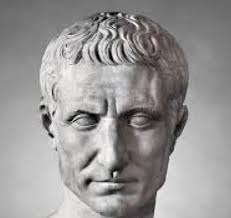
\includegraphics[width=4in, height=3in]{Caesar.jpg}\\
\end{center}

\justifying{Now, fast forward many years. With the amount of computing speed that became available with the invention of computers, the Caesar Cipher and Keyword Shift could be cracked almost instantaneously. This is a huge problem since credit cards and electronic communications rapidly increased in the twentieth century. What happened next changed the security world immensely. In 1970, British mathematician and engineer, James Ellis decided on a new type of algorithm. In contrast with the old algorithms, this new algorithm became much more efficient. His idea used a common lock published to everyone. The sender could lock his/her message in this lock and send it back to the receiver. The receiver only has one key now, which will open every message. The difficulty with Ellis is that he could not formalize a mathematical backing for his idea. Luckily in 1977, three men figured out the mathematical algorithms to make what is now known as RSA work. The men were Ronald Rivest, Adi Shamir, and Leonard Adleman. \par}

\begin{center}
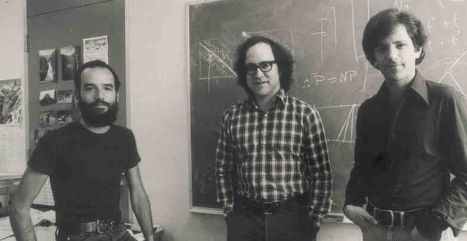
\includegraphics[width=6in, height=3in]{RSA.jpg}\\
\end{center}

\begin{center}
\section{Examples}
\begin{center}
\underline{\textbf{Caesar Cipher}}\\
\justifying{Suppose I want to send the following excerpt from the opening of the classic, ``The Great Gatsby." ``in my younger and more vulnerable years my father gave me some advice that ive been turning over in my mind ever since
whenever you feel like criticizing any one he told me just remember that all the people in this world havent had the advantages that youve had" I have left out punctuation and capitalization for simplicity of the example. Suppose I want to use a shift to the left 4 places. The encrypted message will be, ``mr qc csyrkiv erh qsvi zyprivefpi cievw qc jexliv kezi qi wsqi ehzmgi xlex mzi fiir xyvrmrk sziv mr qc qmrh iziv wmrgi aliriziv csy jiip pmoi gvmxmgmdmrk erc sri li xsph qi nywx viqiqfiv xlex epp xli tistpi mr xlmw asvph lezirx leh xli ehzerxekiw xlex csyzi leh" \par}
\end{center}
\begin{center}
Below is the converted alphabet.\\
\vspace{1.5mm}
\begin{tabular}{|c|c|c|c|c|c|c|c|c|c|c|c|c|c|c|c|c|c|c|c|c|c|c|c|c|c|c|c|c|c|}
\hline
original & a & b & c & d & e & f & g & h & i & j & k & l & m \\
\hline
new & e & f & g & h & i & j & k & l & m & n & o & p & q \\
\hline
original  & n & o & p & q & r & s & t & u & v & w & x & y & z\\
\hline 
new  & r & s & t & u & v & w & x & y & z & a & b & c & d\\
\hline
\end{tabular}\\
Then, I completed a frequency analysis on the encrypted message. The table below shows this analysis.\\
\vspace{1.5mm}
\begin{tabular}{|c|c|c|c|c|c|c|c|c|c|c|c|c|c|c|c|c|c|c|c|c|c|c|c|c|c|c|c|c|c|}
\hline
character & e & f & g & h & i & j & k & l & m & n & o & p & q \\
\hline
number of times appeared & 17 & 3 & 4 & 8 & 36 & 2 & 5 & 12 & 14 & 1 & 1 & 9 & 10 \\
\hline
character &  r & s & t & u & v & w & x & y & z & a & b & c & d\\
\hline
number of times appeared &17 & 10 & 2 & 0 & 13 & 6 & 16 & 6 & 10 & 2 & 0 & 8 & 1\\
\hline
\end{tabular}
\end{center}

\begin{center}
\justifying{Examining the frequency of the characters, I found that I appeared the most often in the encrypted message. I know that the character, e, is the most commonly used letter in the English language. By using this information, I know that the ``i" was most likely the ``e" in the original message. Therefore, the sender must have shifted the original alphabet to the left 4 places. In order to decrypt the message, shift the alphabet to the right 4 places. Converting the encrypted message with this shift 4 places right gives the original message back. in order to have this frequency analysis work well, one must have a sufficiently long message. If I wanted to send a one or two word message using the Caesar Cipher, it is likely that the frequency analysis would not produce an accurate result. \par}
\end{center}
\begin{center}
\underline{\textbf{Example of a Keyword Shift}}\\
\justifying{Suppose I wanted to use a keyword of HelloWorld. I would remove any repeats to begin with. This would simplify the keyword down to helowrd. Below is the alphabet conversion using this keyword shift.  \par}
\begin{center}
\begin{tabular}{|c|c|c|c|c|c|c|c|c|c|c|c|c|c|c|c|c|c|c|c|c|c|c|c|c|c|c|c|c|c|}
\hline
original & a & b & c & d & e & f & g & h & i & j & k & l & m\\
\hline
new & h & e & l & o & w & r & d & a & b & c & f & g & i \\
\hline
original  & n & o & p & q & r & s & t & u & v & w & x & y & z\\
\hline 
new  & j & k & m & n & p & q & s & t & u & v  & x & y & z\\
\hline
\end{tabular}\\
\vspace{1.5mm}
\pagebreak
\begin{center}
\justifying{A similar process would be completed as with the Caesar Cipher. Since the keyword shift is not necessarily preserving the order of the alphabet, the decrypting process will take longer. Although, with a sufficiently long message, a frequency analysis can again be completed to decrypt an encoded message.\par}
\end{center}
\end{center}
\end{center}
\end{center}
\begin{center}
\section{How RSA Works}

\justifying{The following text will show the algorithm for completing an RSA problem. The first steps will result from the receiver, the second set of steps result from the sender, the last set of steps result from the receiver again. An example demonstrating the RSA algorithm will be worked out later in the essay. This example will include small numbers, since the actual algorithm assumes extremely large numbers (100-200 digits long making a product 200-400 digits long).\par}

\justifying{In the RSA process there will be a sender and a receiver. The receiver will begin the process by picking some information, computing some other information, and announcing certain pieces publicly. The sender used the publicly announced information to encode a message in order for a middle man not to intercept and easily decode the message.\par}

\justifying{First, have the receiver pick two very large primes. Call these primes $p$ and $q$. These are usually 100 to 200 digits long. Next, the receiver will compute the product of $p$ and $q$. Call the product $n$. The receiver will also take $p-1$ and $q-1$ then compute the least common multiple of these two values. Call this number $m$. The next step the receiver takes is picking an $e$ relatively prime to $m$. The $e$ value will be the encryption key. Next, the receiver can compute the decryption key, $d$, which comes from solving $ed \mod m=1$. Finally, the receiver will announce the $n$ value and $e$ value publicly.\par}

\justifying{The next steps include the sender encoding a message to give to the receiver. First, the sender has to decide on a message he/she wants to send. Once this is decided upon, the sender must convert the message to a string of digits. One nice way to do this is by giving each letter a two-digit code. For example, A could correspond to 01 as it is the first letter in the alphabet, and Z could correspond to 26 as it is the twenty-sixth letter in the alphabet. The sender can also choose the ways in which to represent a blank. One nice way is with a 00. Once the message is converted into the string of digits, the sender breaks up the message into uniform blocks of digits. We can call these uniform blocks $M_1, M_2, ... , M_k$. If the last string is missing some digits, zeros can be inserted at the end in order to create uniform blocks, but the zeros will simply correspond to blanks, so the message will not be effected. Lastly, for each string, the sender calculates and sends $R_i$ values corresponding to each $M_i$ value. These values are computed as $R_i=M_i^e \mod n$, where $e$ was the encryption key and $n=pq$. These values were the ones announced publicly.\par}

\justifying{Now, the receiver will be acquiring many messages. These messages are each of the $R_i$ values. When receiving these messages, the receiver will compute values for $R_i^d \mod n$. This computation will decrypt the encrypted message that was completed by the sender. After each of the $R_i$ values are decrypted, the strings of digits can be placed in sequence. The receiver then breaks up the long string into blocks of two because each letter is represented with a two-digit code. The receiver finds the letters corresponding to each two-digit code and decrypts the entire original message.\par}
\end{center}


\begin{center}
\underline{\textbf{Example of RSA}}\\
\begin{center}
\justifying{Next, I will complete an example of the RSA encryption and decryption below. The numbers I will use are very small to demonstrate the algorithm without making the computations take several pages just for each number.\par}
\justifying{First, the receiver wants to pick his/her two large primes. In this example, choose $p=37$ and $q=73$. Then, the receiver computes the product of these two numbers. The product is 2701. Call this value $n$. Next, subtract one from each 37 and 73 to get 36 and 72. The least common multiple of these two numbers is computed and called $m$. Thus, $m=72$. The next step for the receiver is to find an encryption key that is relatively prime to 72. For simplicity, choose a small number, say 7. Lastly, the receiver will compute a $d$ value that satisfies $7d \mod 72=1$. The $d$ value satisfying this equation is 31. The receiver announces $n=2701$ and $e=7$ publicly. \par}
\justifying{Consider we are wanting to send a message to the receiver, but we want to encode the message, ``YES." As the sender, let's use the code 01 for A through 26 for Z and 00 for a blank. Converting the Y, we get 25. Converting the E, we get 05, and for converting the S, we get 19. The string of digits is 250519. Now, we will break this up into strings of length 4. We find the strings as 2505 and 1900. We added the extra 00 to the end of 19 to force a string of length four. Next, call $M_1=2505$ and $M_2=1900$. Compute $R_1=2505^7 \mod 2701=692$ and $R_2=1900^7 \mod 2701=1734$. The values 692 and 1734 are now sent to the receiver.\par}
\justifying{Upon receiving these messages, the receiver can add a 0 onto the front of 692 to force a string of length four. Next, the receiver will take $692^{31} \mod 2701=2505$ and $1734^{31} \mod 2701=1900$. Combining these strings, we have 25051900. Since each letter is encoded with a two-digit number, split 25051900 into strings of length two. We get 25, 05, 19, 00. Converting each of these back into a letter, we find 25(Y), 05(E), and 19(S). The original message, ``YES," has how now been found out by the receiver.\par}
\end{center}
\end{center}
\begin{center}
\underline{\textbf{Mod Simplification}}\\
We have just completed an RSA encryption and decryption example. Even when using small numbers, we were dealing with numbers that became very large very quickly. In order to make some of the simplification quicker and more efficient, some modular arithmetic rules can be used in order to simplify the value of $692^{31}$. First, let's use basic exponent rules to simplify $692^{31}=(692^2)^8(692^3)^5$. We have not gone from $692^{31}$, which is almost 100 digits long to $692^2$ and $692^3$, which are six and nine digits long respectively. We then combine these exponent simplifications with modular arithmetic simplifications to find, $692^{31} \mod 2701 \equiv ((692^2 \mod 2701)^8 \mod 2701)\cdot$ $((692^3 \mod 2701)^5 \mod 2701) \mod 2701 $. We can not mod $692^2$ and $692^3$ out by 2701 instead of modding out $692^{31}$ by 2701 all at one time. Both the original and simplified form give the same answer of 2505.

\end{center}
\begin{center}
\section{Proof}
\justifying{Before proving why the RSA algorithm works so well, we need to assume a couple theorems. These are Fermat's Little Theorem and the Chinese Remainder Theorem. \par}
\begin{center}
\underline{\textbf{Fermat's Little Theorem}}\\
If $p$ is any prime number, and $a$ is any integer such that $p \nmid a$, then $a^{p-1}\equiv 1\mod p$.\\
\end{center}
\begin{center}
\underline{\textbf{Chinese Remainder Thoerem}}\\
A system of linear congruences modulo pairwise relatively prime integers has a unique solution modulo the product of these moduli.\\
\end{center}
\justifying{The goal of the proof is to show if we can find a $d$ and if $R$=$M^e \mod n$ then $R^d\equiv M \mod n$. For cleanliness, the subscripts of $R$ and $M$ will be excluded from the proof. The proof starts by assuming we have a $p, q$ prime, $n=pq$, $m=lcm (p-1, q-1)$, and $e$ is relatively prime to $m$. Next, let's assume that we have $de \equiv 1 \mod (p-1)(q-1)$. Then, there must exist an integer, $k$, such that $de=1+k(p-1)(q-1)$. From here, it follows that $R^d\equiv (M^e)^d=M^{de}=M^{1+k(p-1)(q-1)}\mod n$. We know $p$ and $q$ are prime, so the greatest common divisor between    each of them and $M$ is 1. Therefore, by Fermat's Little Theorem $M^{p-1}\equiv 1 \mod p$ and $M^{q-1} \equiv 1 \mod q$. Consequently, $R^d \equiv M \cdot (M^{p-1})^{k(q-1)}\equiv M\cdot 1 = M \mod p$. Similarly, $R^d \equiv M \cdot (M^{q-1})^{k(p-1)}\equiv M\cdot 1 = M \mod q$. Lastly, we know the greatest common divisor of $p$ and $q$ is 1. Thus, by the Chinese Remainder Theorem, $R^d\equiv M\mod pq$.  \par}
\end{center}
The reason this algorithm works so well is that the message being sent is encrypted without some easily identifiable decryption key. In order for a computer to factor some of these large numbers, it would take thousands of years given the brute force methods the computer would use. People do not currently know efficient ways of factoring these large products of two primes. Therefore, there is a high sense of security knowing a message is being sent with information encrypted based on very large prime numbers.
\end{center}

\begin{center}
\underline{\textbf{Future Work}}\\
\justifying{As the descriptions and examples have shown, RSA is based on prime numbers. Since not much is known about the relationships between prime numbers, RSA can fuel research about primes and relationships between them. In order to make the process of RSA quicker, some non-secret form of communication, such as email, could be used to send pieces of information about the encryption. Until 2007, the RSA company gave cash prizes for factoring large numbers into two primes.\par}
\end{center}
\pagebreak
\begin{thebibliography}{99}

\bibitem{Ep} S. Epp, \underline{Discrete Mathematics with Applications 4th Edition}, Brooks/Cole, 2011.
\bibitem{Ga} J. Gallian, \underline{Contemporary Abstract Algebra 8th Edition}, Brooks/Cole, 2013.
\bibitem{Ro} K. H. Rosen, \underline{Discrete Mathematics and Its Applications 7th Edition}, Monmouth University, 2007.
\bibitem{Ha} Public Key Cryptography: RSA Encryption Algorithm, \\ \url{https://www.youtube.com/watch?v=wXB-V_Keiu8}
Princeton University Press, 2008.

\end{thebibliography}
\begin{center}
I have neither given or received, nor have I tolerated others' use of unauthorized aid. 
\end{center}
\end{document}